% begin module first-derivative-up-down
\begin{frame}
\frametitle{What Does $f'$ Say About $f$?}
\begin{columns}[c]
\column{.4\textwidth}
\ 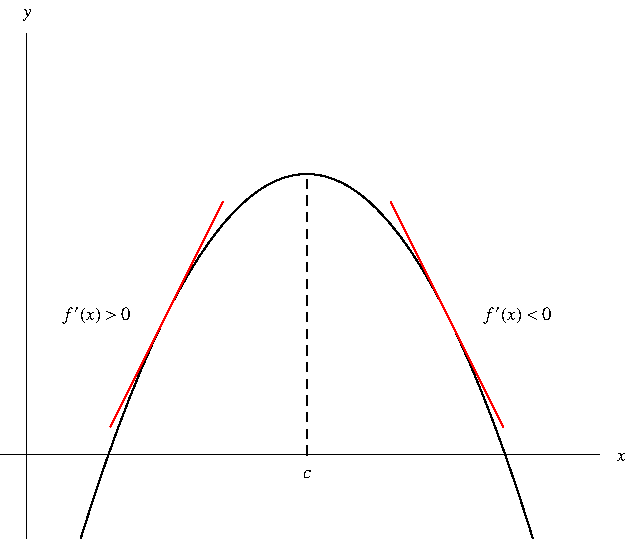
\includegraphics[height=4cm]{curve-sketching/pictures/04-03-firstderiva.pdf}%
\column{.6\textwidth}
\begin{itemize}
\item  Consider the graph on the left. 
\item  $f'(x) > 0$ to the left of $c$ and $f'(x) < 0$ to the right of $c$.
\item  $f$ is increasing to the left of $c$ and decreasing to the right of $c$.
\item<2->  This property holds more generally:
\end{itemize}
\end{columns}
\uncover<2->{Increasing/Decreasing Test}
\begin{enumerate}
\item<2->  If $f'(x) > 0$ on an interval, then $f$ is increasing on that interval.
\item<2->  If $f'(x) < 0$ on an interval, then $f$ is decreasing on that interval.
\end{enumerate}
\end{frame}
% end module first-derivative-up-down
